\subsection{Classical NLP for factor investing}

% 
% Version: 1.0.5
% Last updated: 2026-07-21
% Versioning scheme:
%   MAJOR: structural overhaul, renumbering of top-level sections, new Parts
%   MINOR: new section, new figure, new content batch, new vendor table column
%   PATCH: prose tweaks, citation additions, single-bib-entry fixes, typo fixes
% See `VERSIONING_ch20.md` in chapter folder for the change log.
% Provenance: this chapter is the first of five chapters in Part V of the
% 2nd edition, extracted from the monolithic Chapter_20_Draft19.md
% (v3.9.7, 48,526 words, archived in `_archive_monolithic_v3.9.7/`).
%

\subsubsection{Introduction}

The preceding chapters of this book have explored a wide array of machine learning tools for factor investing, from penalized regressions (Chapter 5) and tree-based models (Chapter 6) to neural networks (Chapter 7), reinforcement learning (Chapter 16), and genetic algorithms (Chapter 19). All of these methods operate on the same type of input: structured, numerical data organized into a matrix of firm characteristics. The book's standard dataset of 1,207 US stocks with 93 features (see Chapter 1) epitomizes this paradigm. Yet a vast reservoir of economically relevant information is encoded not in numbers but in words.

Corporate filings, earnings call transcripts, analyst reports, news articles, central bank communications, and social-media posts contain forward-looking statements, managerial tone, risk disclosures, and sentiment cues that are difficult (and often impossible) to capture through numerical characteristics alone. The field of \textit{natural language processing} (NLP) provides the tools to convert this unstructured text into quantitative signals suitable for factor models and portfolio construction.

The relevance of text for asset pricing is well established empirically. Earlier foundations were laid by \cite{antweiler2004internet}, who showed that the volume and disagreement of Internet stock message board posts predict next-day volatility and trading activity, and by \cite{das2007yahoo}, who classified Yahoo! Finance messages about 24 technology stocks and found that aggregate sentiment tracks intraday returns. Building on this foundation, \cite{tetlock2007giving} showed that the fraction of negative words in a Wall Street Journal column predicted next-day Dow Jones returns. \cite{loughran2011liability} demonstrated that generic sentiment dictionaries misclassify financial language and proposed a domain-specific lexicon that has since become the standard.

This chapter focuses on the \textit{classical} NLP toolkit that has driven text-based factor research for two decades, and that remains the right starting point for any production pipeline. We introduce text as a data class and survey the six source families that recur throughout Part V (Section 20.2), define the preprocessing and bag-of-words representations that every downstream method consumes (Section 20.3), develop the dictionary-based sentiment scoring that opened the field empirically (Section 20.4), introduce topic models for thematic factor discovery (Section 20.5), present named-entity recognition and event extraction for event-driven strategies (Section 20.6), and close with the two factor families that the classical toolkit has produced in mature, peer-reviewed form: disclosure-based factors (Section 20.7) and news and media-flow factors (Section 20.8). The remainder of the NLP toolkit (embeddings, transformers, large language models, and an end-to-end case study) is deferred to the following chapters.

NLP for equity markets is now a vast and rapidly growing literature: corpus surveys identify on the order of 1,000 or more papers since the late 2000s, with roughly 76\% appearing after 2021 alone \citep{lis2024investor}. Two structural axes organize the field. The first is a \textit{method curve} that runs from rule-based lexicons through classical machine learning and dense embeddings to BERT-style encoders and, finally, generative LLMs; \cite{mishev2020evaluation} provide the canonical benchmark spanning this entire arc, testing approximately 30 sentiment models on financial text and finding that transformers dominate accuracy while sacrificing transparency. The second is a \textit{source curve}: early studies focused on news articles and message boards because they are short and syntactically simple, while longer and more specialized documents such as earnings-call transcripts and 10-K filings only became tractable once transformer-scale encoders arrived around 2019-2020.
Two caveats are in order. First, the book's standard \texttt{mlfi\_us\_data} panel is numerical only: it does not contain textual data, in keeping with the design of the dataset described in Chapter 1. Shipping a raw text corpus alongside this book would be problematic on two counts. Legally, although individual corporate filings, earnings-call transcripts, and news articles are public, their bulk redistribution sits in a grey zone: publishers and transcript vendors retain copyright on the typeset record, and SEC filings are public but not licence-free when repackaged at scale. Practically, assembling a research-grade corpus of millions of filings, transcripts, and news items is an engineering project (storage, deduplication, OCR for older filings, ticker mapping, point-in-time alignment) that is well outside the scope of a methods textbook. To mitigate both concerns we ship a \textit{sentiment-derived} companion dataset rather than the raw text itself: for the 437 largest US stocks in \texttt{mlfi\_us\_data} we processed the full available history of quarterly earnings-call transcripts and recorded the per-call sentiment scores produced by each of the model families introduced across Part V (classical dictionaries, contextual encoders, and an LLM-based scorer), split into prepared-remarks, Q\&A-management, and Q\&A-analyst buckets. Distributing scores rather than text sidesteps the licensing question and shrinks the artifact from terabytes to a single panel CSV. The empirical tables of Chapter 21 and the case study of Chapter 24 read from this companion panel directly; the methodology subsections of the present chapter use much shorter illustrative samples (a single Coca-Cola Q1 2026 transcript excerpt and a handful of stylised sentences) when the pedagogical point is the technique itself rather than its cross-sectional performance. Second, NLP is a vast and fast-moving field. We do not attempt encyclopedic coverage; instead, we focus on the methods most directly relevant to equity factor investing and refer the interested reader to \cite{jurafsky2024speech} for a comprehensive treatment of the broader NLP landscape, and to the finance-specific survey of \cite{xing2018natural}, which catalogues the text sources (news, filings, message boards, social media), modeling families (lexicon, statistical, deep learning), and applications (return and volatility forecasting, event studies) that underpin the literature Part V draws on.

\textbf{A note on notation in this chapter.} Several equations in this chapter use letters that double as both NLP and asset-pricing indices. We highlight the local redefinitions to avoid confusion. In Equation (20.7), $n$ indexes word positions within a document (not assets) and $N_d$ is the document length. In Equation (20.8), $t$ indexes corpus tokens and $T$ the corpus length (not calendar time). The symbol $\alpha$ appears in two distinct roles: a Dirichlet concentration vector in Equation (20.7) and a portfolio intercept in Equation (20.13); context disambiguates in each case. We retain these letter choices because they are standard in the NLP literature, but we flag them here so that the cross-reference to Chapter 1's notation is unambiguous.

\subsubsection{Text as a data class}

Text differs from the structured numerical features of Chapters 2 through 19 in three ways that drive every design choice that follows. It is \textit{high-dimensional}: a typical 10-K contains 50,000 to 150,000 tokens (the atomic word or word-piece units a text is broken into, defined precisely in Section 20.3.1) drawn from a vocabulary of tens of thousands of distinct types, so any representation must compress aggressively before reaching a tractable feature space. It is \textit{semantic}: identical numbers (``revenue grew 5\%'') carry very different signals depending on the surrounding context (guidance versus historical, prepared remarks versus Q\&A, peer comparison versus stand-alone), so encodings that ignore surrounding context (the classical bag-of-words representation defined in Section 20.3.2, which simply counts how often each word appears) throw away information that the contextual encoders of Chapter 22 (transformer models whose representation of each word depends on the entire sentence) preserve. And it is \textit{irregularly timed}: filings appear on quarterly schedules with embargoed release windows, earnings calls are clustered in two-week reporting waves, news arrives continuously with intra-day spikes, and social-media posts arrive in bursts driven by events; this temporal heterogeneity dictates how text-derived features should be aligned to the monthly factor frequency of the book's dataset.

These three properties motivate a \textit{data-class} view of text. Rather than treating ``text'' as a single source, we partition the universe of financial text into six classes that differ along the dimensions that matter for factor investing: producer (firm, analyst, journalist, regulator, retail investor), publication frequency, regulatory status, signal-to-noise ratio, coverage breadth, and typical document length. Each class supports a distinct set of metrics and a distinct set of factor strategies, and each has accumulated its own peer-reviewed empirical literature.
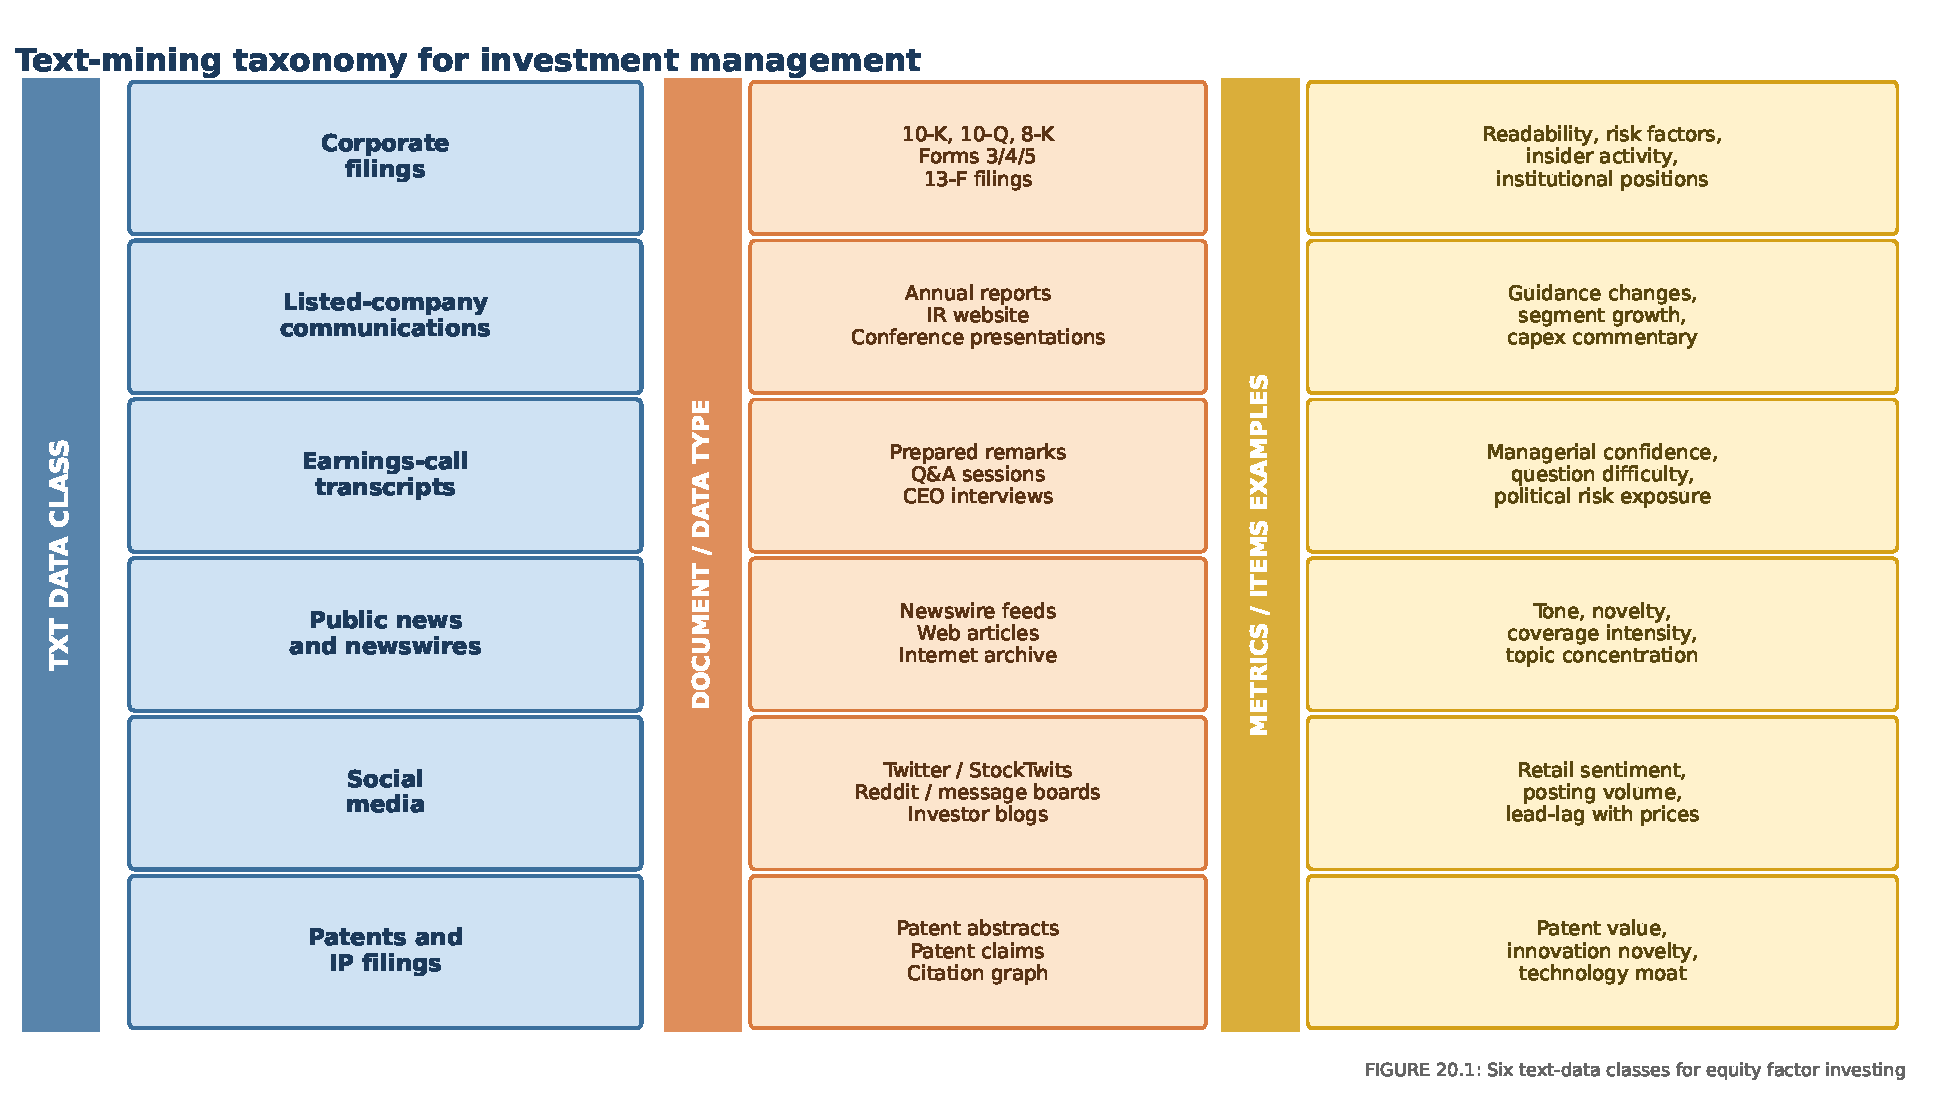
\includegraphics[width=0.7\linewidth]{files/figure_20_1_taxonomy-b9a4f75ffab7a7164fe7d0585f2b1dd1.pdf}

FIGURE 20.1 organizes the six text-data classes along three axes (data class, document or data type, metrics or items examples) following the standard practitioner taxonomy used in industry research. We now describe each row in turn, summarizing what the class is, who produces it, what use cases it enables, and which published evidence anchors it in the empirical literature.

\paragraph{Corporate filings (10-K, 10-Q, 8-K, Forms 3/4/5, 13-F)}

Filings submitted to the U.S. Securities and Exchange Commission are the most regulated text class in the financial system. The annual 10-K and quarterly 10-Q reports contain audited financial statements wrapped in extensive textual discussion, including the Management's Discussion and Analysis (MD\&A), risk factors, and forward-looking statements. The 8-K reports material events as they occur; Forms 3, 4, and 5 disclose insider transactions; and 13-F filings reveal quarterly institutional positions above the reporting threshold. These documents are long (typically 100 to 300 pages for a 10-K), uniformly formatted, infrequent (quarterly to annual), and legally vetted, which makes them high-signal but slow-moving. The classical evidence on filings runs through \cite{loughran2011liability}, whose finance-specific sentiment dictionary corrects the systematic misclassification of generic lexicons on legal and accounting prose; \cite{li2008annual}, who showed that 10-K readability (Fog index) predicts earnings persistence; \cite{cohen2020lazy}, who documented the Lazy Prices anomaly whereby year-over-year textual changes in 10-Ks generate a long-short return of roughly 23.5\% per annum; \cite{bushee2018linguistic}, who decompose linguistic complexity into obfuscation and information components; \cite{hoberg2016text}, who build text-based industry classifications from 10-K product descriptions; \cite{campbell2014information}, who quantify the information content of mandatory risk factor disclosures; and \cite{lopezlira2023risk}, who extracts risk factors directly from 10-K text and prices them in the cross-section.

\paragraph{Listed-company communications (annual reports, IR websites, conference presentations)}

Beyond mandatory SEC filings, listed companies maintain a parallel stream of voluntary communications: glossy annual reports, investor-relations website content, sustainability reports, capital-markets-day decks, and conference presentations to sell-side analysts. These materials are less constrained by accounting standards but governed by Regulation Fair Disclosure, which prohibits selective release of material information. They are useful for extracting forward-looking commentary that is downplayed or absent in SEC filings: total addressable market estimates, net sales by geography and product segment, segment-level growth narratives, capex guidance, and product-pipeline disclosures. The empirical evidence here is thinner than for SEC filings but growing: \cite{sautner2023firm} construct firm-level climate change exposure measures by combining earnings calls with IR communications, and \cite{webersinke2022climatebert} pretrain ClimateBERT on a large corpus of corporate sustainability reports and use it to score voluntary climate disclosures across firms.

\paragraph{Earnings call transcripts}

Quarterly earnings conference calls are perhaps the richest single-source text class for equity factor investing. Each call has two parts with very different information content: prepared remarks (10 to 30 minutes), in which management reads a scripted account of the quarter, and the Q\&A session (typically 30 to 60 minutes), in which sell-side analysts question executives in real time. Transcripts are publicly available with a delay measured in hours and cover essentially every US-listed company that holds a quarterly earnings call. \cite{larcker2012detecting} identified linguistic markers of deceptive language by executives who subsequently restated earnings; \cite{hassan2019politicalrisk} extracted firm-level political risk scores from transcripts that load on lobbying activity and predict the cross-section of returns; \cite{sautner2023firm} measured climate exposure at the firm level; \cite{kim2024transcripts} used a generative LLM to distil firm-level risk assessments from earnings-call transcripts that explain return volatility and firms' risk-mitigating actions better than dictionary-based measures; \cite{hafez2021transcripts} showed that document sentiment, event sentiment, and disclosure transparency are three largely orthogonal signals extractable from the same transcript; \cite{zhao2018alpha} demonstrated that the Q\&A portion of the call carries substantially more cross-sectional alpha than the prepared remarks; and \cite{yang2020html} introduced HTML, the hierarchical transformer architecture that has since become standard for long-form transcript modeling.

\paragraph{Public news and newswires}

News is the most-studied text class in the literature and the dominant data source in every method era surveyed by \cite{mishev2020evaluation}. It is heterogeneous in publisher (Wall Street Journal, Reuters, Dow Jones, Bloomberg, regional newspapers, financial blogs), frequency (intra-day to daily), and coverage (broad market commentary versus firm-specific news). The canonical empirical results start with \cite{tetlock2007giving}, who showed that the negative-word share in a single daily WSJ column predicts next-day Dow returns; \cite{tetlock2008more}, who generalized the finding to firm-specific news; \cite{antweiler2004internet} on Internet message-board volumes; \cite{engelberg2011causal}, who isolated the \textit{causal} effect of local newspaper coverage on local trading via weather-driven distribution disruptions; \cite{hillert2014media}, whose interaction of past returns with press coverage drives the momentum factor; \cite{heston2017news}, who built a news-tone factor not subsumed by price momentum; \cite{garcia2013sentiment} on the recession-dependence of news sentiment effects; \cite{calomiris2019news} on novelty-weighted sentiment in a 51-country sample; \cite{manela2017news}, who construct the NVIX disaster-concerns index from front-page articles since 1890; and \cite{ke2019predicting}, who push the out-of-sample (OOS) predictive frontier with their SESTM (Sentiment Extraction via Screening and Topic Modeling) supervised text learner over Dow Jones news. Two early methodological studies anchor the historical foundation of the literature for this data class: \cite{devitt2007sentiment}, working with cohesion-based analysis of financial news, were among the first to demonstrate rigorously that textual tone carries price-relevant information beyond prices themselves, and \cite{schumaker2012evaluating}, in one of the canonical early studies in \textit{Decision Support Systems}, showed that lexicon-based sentiment over news articles produces reliable predictive signals for stock returns.

\paragraph{Social media (Twitter/X, StockTwits, Reddit, message boards)}

Social media is the youngest and noisiest text class in the taxonomy, characterised by very short documents (Twitter's 280-character limit), heavy slang and emoji usage, severe class imbalance (most posts are neutral chatter), and intermittent retail-sentiment regimes that can shift abruptly during specific events (GameStop 2021, AMC 2021, COVID 2020). Despite these challenges, peer-reviewed evidence on its information content is robust: \cite{bollen2011twitter} reported aggregate Twitter mood as a leading indicator of DJIA moves; \cite{chen2014wisdom} used Seeking Alpha posts to predict next-quarter earnings; \cite{bartov2018twitter} showed that pre-announcement Twitter sentiment predicts both earnings surprises and announcement-day returns, particularly for low-coverage names; \cite{xu2018stock} released the StockNet dataset (88 stocks, two years of tweets and prices) that has become a standard NLP benchmark; \cite{zheludev2014when} provide a negative-control finding that the lead-lag effect of Twitter on the S\&P 500 is detectable for high-volume cashtags but absent at the aggregate index level; \cite{sawhney2020deep} introduced graph-attention models that combine tweet content with inter-company correlation graphs; and \cite{albladi2025twitter} survey the post-transformer state of the art across the broader Twitter sentiment literature.

\paragraph{Patents and intellectual property filings}

The final class in our taxonomy, patents, is the least developed in the equity factor investing literature but is included here because it sits at the intersection of two robust signals: corporate R\&D effort (a quality factor proxy) and innovation novelty (an asset-pricing factor in its own right). Patent abstracts describe what the invention does, patent claims define what is legally protected, and the patent citation graph captures intellectual debt and influence. Useful firm-level metrics derived from patent text include the patent-family size (how broadly an invention is protected internationally), expiration timelines (which affect future cash flows), novelty keywords (which proxy for breakthrough innovation), the count of citing patents (an empirical proxy for technology-moat strength), and concept exposure to specific technology themes. The flagship paper in this area, \cite{kogan2017technological}, measures patent value from text and shows that text-derived novelty predicts future cash flows and stock returns; although outside the dominant news and transcript literature of this chapter, the methodology is a natural extension of the techniques developed in Sections 20.3 through 20.7 and an open avenue for factor researchers working at the intersection of IP economics and asset pricing.

\subsubsection{Text as data: preprocessing and representation}

\paragraph{From raw text to clean tokens}

Before any quantitative analysis can begin, raw text must be transformed into a structured representation. This preprocessing pipeline is the foundation of all NLP methods, classical and modern alike, and its quality directly affects downstream performance. We outline the standard steps below.

\textbf{Tokenization} is the process of splitting a string of text into individual units called \textit{tokens}. In the simplest case, tokens are words separated by whitespace, but financial text often requires more nuanced treatment. Consider the string \texttt{"Q3 2023 EPS beat by \$0.12"}: a naive whitespace tokenizer would treat \texttt{"\$0.12"} as a single token, while a more sophisticated tokenizer might separate the currency symbol from the number. The \texttt{nltk} library provides several tokenizers suited to different use cases.

\begin{verbatim}
import nltk
nltk.download('punkt_tab', quiet=True)
sentence = "EPS of $0.86 increased 18% year-over-year, helped by 3% currency tailwinds."
print(nltk.word_tokenize(sentence))      # NLTK splits punctuation from numbers
\end{verbatim}

\begin{verbatim}
['EPS', 'of', '$', '0.86', 'increased', '18', '%', 'year-over-year', ',', 'helped', 'by', '3', '%', 'currency', 'tailwinds', '.']
\end{verbatim}

The tokenizer isolates the dollar sign and the percent sign as their own tokens, which is useful for a downstream rule that wants to identify currency or magnitude expressions, but it also splits \texttt{"18"} from \texttt{"\%"}, so any pipeline that wants the original \texttt{"18\%"} magnitude back must reassemble adjacent tokens (or use a custom regular-expression tokenizer).

\textbf{Stop-word removal} eliminates high-frequency words that carry little semantic content: ``the,'' ``is,'' ``and,'' ``of.'' Removing these words reduces the dimensionality of the representation and focuses subsequent analysis on content-bearing terms. However, in financial text, some seemingly generic words can carry meaning (e.g., ``will'' in forward-looking statements), so the choice of stop-word list requires domain judgment.

\begin{verbatim}
from nltk.corpus import stopwords
nltk.download('stopwords', quiet=True)
stop = set(stopwords.words('english'))
sentence = "We are continuing to judiciously manage our balance sheet as we await a court decision."
tokens = [t for t in nltk.word_tokenize(sentence.lower()) if t.isalpha()]
print([t for t in tokens if t not in stop])
\end{verbatim}

\begin{verbatim}
['continuing', 'judiciously', 'manage', 'balance', 'sheet', 'await', 'court', 'decision']
\end{verbatim}

Eight content-bearing tokens survive out of seventeen original tokens. The pronouns (``we,'' ``our''), auxiliaries (``are,'' ``to,'' ``as''), and the article (``a'') are dropped; ``balance sheet'' and ``court decision'' survive as the substantive concepts.

\textbf{Stemming and lemmatization} reduce words to their root forms. Stemming applies crude suffix-stripping rules (``running'' becomes ``run,'' ``consolidation'' becomes ``consolid''), while lemmatization uses morphological analysis to produce valid dictionary forms (``better'' becomes ``good,'' ``are'' becomes ``be''). For financial applications, lemmatization is generally preferred because it preserves interpretability: ``diversified'' and ``diversification'' both reduce to ``diversify'' rather than the truncated stem ``diversif.''

\begin{verbatim}
from nltk.stem import WordNetLemmatizer, PorterStemmer
nltk.download('wordnet', quiet=True)
lem, stem = WordNetLemmatizer(), PorterStemmer()
words = ['consumers', 'monitored', 'preferring', 'flavors', 'evenings', 'better']
print('lemmas:', [lem.lemmatize(w) for w in words])
print('stems :', [stem.stem(w) for w in words])
\end{verbatim}

\begin{verbatim}
lemmas: ['consumer', 'monitored', 'preferring', 'flavor', 'evening', 'better']
stems : ['consum', 'monitor', 'prefer', 'flavor', 'even', 'better']
\end{verbatim}

Lemmatization keeps real dictionary words but only normalises plurals (\texttt{consumers \rightarrow consumer}) unless we pass the right part-of-speech tag for verbs; the Porter stemmer is more aggressive and collapses inflections but produces non-words such as \texttt{consum} and \texttt{even}. Neither method handles \texttt{better \rightarrow good} without a richer morphological resource (NLTK's WordNet lemmatizer with \texttt{pos='a'} would).

\textbf{Handling financial jargon.} Domain-specific vocabulary poses particular challenges. Ticker symbols (AAPL, MSFT), financial abbreviations (EPS, EBITDA, P/E), and compound terms (free-cash-flow, mark-to-market) require custom tokenization rules. Negation handling is especially important: ``not profitable'' should not be treated as two independent tokens in a bag-of-words model. We discuss this further in Section 20.4.3.

\begin{verbatim}
import re
sentence = "Free cash flow was approximately $1.8 billion year-over-year, with no signs of slowing demand."
protect = {'free cash flow': 'free_cash_flow',           # compound term
           'year-over-year': 'year_over_year',           # hyphenated metric
           'no signs of slowing': 'NEG_slowing'}         # negation scope
for src, tgt in protect.items():
    sentence = re.sub(src, tgt, sentence, flags=re.IGNORECASE)
print(nltk.word_tokenize(sentence))
\end{verbatim}

\begin{verbatim}
['free_cash_flow', 'was', 'approximately', '$', '1.8', 'billion', 'year_over_year', ',', 'with', 'NEG_slowing', 'demand', '.']
\end{verbatim}

The substitution pass collapses multi-word financial terms into single tokens before the generic tokenizer runs, preserving them as atomic units downstream. The negation cue is rewritten with a \texttt{NEG\_} prefix on the modified word, so that a bag-of-words sentiment scorer that does not understand syntax still sees \texttt{NEG\_slowing} as a distinct feature rather than positive \texttt{slowing} plus a discarded \texttt{no}.

We illustrate the preprocessing pipeline on six real excerpts taken from the Coca-Cola Q1 2026 earnings call transcript (Coca-Cola, henceforth referenced by its NYSE ticker KO). In practice, the corpus would consist of thousands of 10-K filing excerpts, earnings call paragraphs, or news articles; here a single call already shows the variety of language a sentiment pipeline must cope with.

\begin{verbatim}
import nltk                                          # NLP toolkit
from nltk.corpus import stopwords
from nltk.stem import WordNetLemmatizer
nltk.download('punkt_tab', quiet=True)
nltk.download('stopwords', quiet=True)
nltk.download('wordnet', quiet=True)

documents = [                                        # KO Q1 2026 excerpts
    "We delivered strong first quarter results despite a complex external environment.",
    "Many consumers remain under pressure due to persistent inflation and greater macroeconomic uncertainty.",
    "We harnessed the power of our brands to deliver three percent volume growth across all segments.",
    "Management expects organic revenue growth on track with our full year guidance.",
    "The softness in price mix was attributed to Easter timing and unfavorable category mix from packaged water.",
    "Innovation contributed strongly to revenue growth with Coca Cola Cherry and Diet Coke Cherry powering volume.",
]

lemmatizer = WordNetLemmatizer()
stop_words = set(stopwords.words('english'))

def preprocess(text):
    """Tokenize, lowercase, remove stop words, lemmatize."""
    tokens = nltk.word_tokenize(text.lower())        # Tokenize and lowercase
    tokens = [t for t in tokens if t.isalpha()]       # Keep alphabetic tokens only
    tokens = [t for t in tokens if t not in stop_words]  # Remove stop words
    tokens = [lemmatizer.lemmatize(t) for t in tokens]   # Lemmatize
    return tokens

processed = [preprocess(doc) for doc in documents]
for i, tokens in enumerate(processed):
    print(f"Doc {i}: {tokens}")
\end{verbatim}

\begin{verbatim}
Doc 0: ['delivered', 'strong', 'first', 'quarter', 'result', 'despite', 'complex', 'external', 'environment']
Doc 1: ['many', 'consumer', 'remain', 'pressure', 'due', 'persistent', 'inflation', 'greater', 'macroeconomic', 'uncertainty']
Doc 2: ['harnessed', 'power', 'brand', 'deliver', 'three', 'percent', 'volume', 'growth', 'across', 'segment']
Doc 3: ['management', 'expects', 'organic', 'revenue', 'growth', 'track', 'full', 'year', 'guidance']
Doc 4: ['softness', 'price', 'mix', 'attributed', 'easter', 'timing', 'unfavorable', 'category', 'mix', 'packaged', 'water']
Doc 5: ['innovation', 'contributed', 'strongly', 'revenue', 'growth', 'coca', 'cola', 'cherry', 'diet', 'coke', 'cherry', 'powering', 'volume']
\end{verbatim}

The preprocessing reduces each sentence to its content-bearing lemmas. Notice that ``consumers'' becomes ``consumer,'' ``results'' becomes ``result,'' and common words like ``the,'' ``a,'' ``by'' are removed. The plural ``segments'' is normalised to ``segment,'' and the proper nouns ``Coca,'' ``Cola,'' ``Cherry,'' and ``Coke'' survive as lowercase tokens that a downstream entity-recognition pass (Section 20.6) would tag back as brand names. The resulting token lists are the raw material for the bag-of-words representation introduced in the next subsection.

\paragraph{Bag-of-words and term frequency}

The simplest numerical representation of a text document is the \textit{bag-of-words} (BoW) model: a vector whose length equals the vocabulary size $V$ and whose $k$-th entry counts how many times word $k$ appears in the document. This representation discards word order entirely, treating ``the dog bit the man'' and ``the man bit the dog'' identically.

Let $d$ denote a document and $\mathcal{V} = \{w_1, \ldots, w_V\}$ the vocabulary. The raw term-frequency vector is:

\begin{equation}
\text{tf}(w_k, d) = \frac{\text{count}(w_k, d)}{\sum_{j=1}^{V} \text{count}(w_j, d)}
\tag{20.1}
\end{equation}

where $\text{count}(w_k, d)$ is the number of occurrences of word $w_k$ in document $d$.

Given a corpus of $D$ documents, the \textit{document-term matrix} (DTM) $\mathbf{X} \in \mathbb{R}^{D \times V}$ stores the term frequencies (or raw counts) for all documents. Each row is a document, each column is a word. This matrix is typically very sparse, because any single document uses only a small fraction of the total vocabulary.

Raw term frequency overweights common words. The \textit{term frequency-inverse document frequency} (TF-IDF) weighting addresses this by down-weighting terms that appear in many documents:

\begin{equation}
\text{tf-idf}(w_k, d) = \text{tf}(w_k, d) \times \log \frac{D}{\text{df}(w_k)}
\tag{20.2}
\end{equation}

where $\text{df}(w_k)$ is the number of documents containing word $w_k$. The logarithmic term penalizes words that appear across most documents (e.g., ``company,'' ``quarter'') while boosting words that are distinctive to a few documents (e.g., ``goodwill impairment,'' ``FDA approval''). TF-IDF is arguably the most widely used text representation in applied finance, owing to its simplicity and effectiveness.

We now construct the TF-IDF matrix from the same six KO Q1 2026 excerpts preprocessed above.

\begin{verbatim}
from sklearn.feature_extraction.text import TfidfVectorizer

vectorizer = TfidfVectorizer(
    tokenizer=preprocess,                            # custom preprocessor from §20.3.1
    token_pattern=None,                              # disable default pattern
    max_features=30)                                 # limit vocabulary for display
tfidf_matrix = vectorizer.fit_transform(documents)
feature_names = vectorizer.get_feature_names_out()

# The full 6 x 30 matrix is very sparse: print only the top 4 highest-weighted
# terms per document, which is the empirically useful view of TF-IDF.
for i, row in enumerate(tfidf_matrix.toarray()):
    pairs = sorted(zip(feature_names, row), key=lambda x: -x[1])
    top4  = [f'{t} ({w:.2f})' for t, w in pairs[:4] if w > 0]
    print(f'Doc {i}: ' + ', '.join(top4))
\end{verbatim}

\begin{verbatim}
Doc 0: complex (0.41), delivered (0.41), despite (0.41), environment (0.41)
Doc 1: consumer (0.45), due (0.45), greater (0.45), inflation (0.45)
Doc 2: across (0.44), brand (0.44), deliver (0.44), harnessed (0.44)
Doc 3: expects (0.49), full (0.49), guidance (0.49), revenue (0.40)
Doc 4: mix (0.76), attributed (0.38), category (0.38), easter (0.38)
Doc 5: cherry (0.64), coca (0.32), contributed (0.32), diet (0.32)
\end{verbatim}

The full 6 by 30 TF-IDF matrix is extremely sparse, since each document uses only a small fraction of the vocabulary; the per-document top-4 view above is the empirically useful summary. The highest-weighted terms are those that are both frequent within a document and rare across the corpus. Doc 4 illustrates the construction cleanly: ``mix'' appears twice in that single document and nowhere else in the corpus, so it dominates the row with a weight of 0.76. Doc 5 is similar for ``cherry'', which appears twice in Doc 5 alone. The macroeconomic vocabulary of Doc 1 (``consumer'', ``inflation'', ``greater'', ``due'') and the forward-looking vocabulary of Doc 3 (``expects'', ``full'', ``guidance'') split cleanly along the prepared-remarks-versus-outlook axis that the chapter exploits throughout.

This representation, while simple, already captures meaningful structure. Documents about cash flows (Doc 2, Doc 4) share the terms ``cash'' and ``flow,'' while documents about losses (Doc 1) and earnings beats (Doc 5) are clearly separated. The challenge, of course, is that bag-of-words ignores word order and context entirely, a limitation we address in the sections that follow.

\subsubsection{Sentiment analysis with dictionaries}

\paragraph{The lexicon approach}

The most direct way to extract economic meaning from text is \textit{sentiment analysis}: classifying the tone of a document as positive, negative, or neutral. The simplest and most widely used approach in finance relies on pre-compiled \textit{sentiment dictionaries} (also called lexicons): curated lists of words labeled with their emotional or evaluative polarity.

Early work in computational linguistics used general-purpose lexicons such as the Harvard General Inquirer (GI), which classifies English words into psychological categories including positive and negative tone. \cite{loughran2011liability} showed that general-purpose lexicons perform poorly on financial text. Almost three-quarters of the words classified as ``negative'' by the Harvard GI are not negative in a financial context. The word ``tax,'' for instance, is labeled negative by the GI, yet it carries no evaluative tone in an earnings report. Similarly, ``liability,'' ``cost,'' and ``capital'' are flagged as negative despite being neutral financial terminology.

The \textbf{Loughran-McDonald (LM) dictionary} was specifically constructed for financial documents. The authors analyzed 10-K filings from 1994 to 2008 and identified six sentiment categories: \textit{negative}, \textit{positive}, \textit{uncertainty}, \textit{litigious}, \textit{strong modal}, and \textit{weak modal}. The negative word list (containing terms such as ``loss,'' ``impairment,'' ``decline,'' ``adverse,'' ``default'') has become the de facto standard for financial sentiment analysis. Subsequent studies have largely confirmed that domain-specific dictionaries outperform generic ones for financial text; the survey by \cite{kearney2014textual} provides a thorough review of these findings.

Given a dictionary with positive word set $\mathcal{P}$ and negative word set $\mathcal{N}$, the simplest sentiment score for a document $d$ is the \textit{net tone}:

\begin{equation}
\text{Tone}(d) = \frac{\#(d \cap \mathcal{P}) - \#(d \cap \mathcal{N})}{\#(d \cap \mathcal{P}) + \#(d \cap \mathcal{N})}
\tag{20.3}
\end{equation}

where $\#(d \cap \mathcal{P})$ counts the number of words in $d$ that belong to the positive list. This score ranges from -1 (entirely negative) to +1 (entirely positive). Alternative normalizations divide by total word count rather than the sum of sentiment words, but Equation (20.3) is the most common in the literature. \cite{jegadeesh2013word} showed that giving every LM-listed word equal weight in this formula is suboptimal, because some terms carry much stronger return-predictive content than others. They proposed a market-based term-weighting scheme that estimates each word's informativeness from its association with stock returns around 10-K filing dates, and reported that this data-driven weighting materially improves the out-of-sample predictive power of the tone score relative to the uniform weighting implicit in Equation (20.3).

We demonstrate the Loughran-McDonald approach using six sentences in the style of (and partly drawn from) the KO Q1 2026 earnings call already introduced in Section 20.3.1. In practice, researchers download the LM dictionary from the authors' website and apply it to large corpora of filings or news articles.

\begin{verbatim}
import numpy as np

# Loughran-McDonald word lists (abbreviated for illustration)
lm_positive = {
    'achieve', 'advancement', 'benefit', 'creative', 'efficient', 'enhance',
    'excellent', 'favorable', 'gain', 'great', 'improve', 'improvement',
    'innovation', 'opportunity', 'outstanding', 'positive', 'profitability',
    'progress', 'strength', 'strong', 'succeed', 'success', 'superior'
}
lm_negative = {
    'adverse', 'against', 'closure', 'decline', 'default', 'deficit',
    'deterioration', 'downturn', 'failure', 'impairment', 'inability',
    'litigation', 'loss', 'losses', 'negative', 'penalty', 'restructuring',
    'risk', 'terminate', 'threat', 'unfavorable', 'volatility', 'weakness'
}

sample_texts = [                                     # KO-flavored excerpts
    "Revenue growth was strong driven by innovation across our beverage portfolio.",
    "The softness in price mix was attributed to unfavorable category mix and constrained production capacity.",
    "Operating losses did not materialize, and margins held firm.",
    "Free cash flow improved and management sees favorable conditions for the remainder of the year.",
    "Adverse macroeconomic conditions and persistent inflation pose a risk to near-term consumer demand.",
    "The firm achieved outstanding results with superior margin expansion in North America.",
]
\end{verbatim}

\begin{verbatim}
def lm_sentiment(text, pos_words, neg_words):
    """Compute Loughran-McDonald net tone for a text."""
    tokens = set(text.lower().split())               # Simple whitespace tokenizer
    n_pos = len(tokens & pos_words)                  # Count positive matches
    n_neg = len(tokens & neg_words)                  # Count negative matches
    denom = n_pos + n_neg
    if denom == 0:
        return 0.0
    return (n_pos - n_neg) / denom                   # Net tone in [-1, 1]

scores = [lm_sentiment(t, lm_positive, lm_negative) for t in sample_texts]
for i, (text, score) in enumerate(zip(sample_texts, scores)):
    label = "Positive" if score > 0 else ("Negative" if score < 0 else "Neutral")
    print(f"Doc {i} ({label:>8s}, tone={score:+.2f}): {text[:60]}...")
\end{verbatim}

\begin{verbatim}
Doc 0 (Positive, tone=+1.00): Revenue growth was strong driven by innovation across our...
Doc 1 (Negative, tone=-1.00): The softness in price mix was attributed to unfavorable cat...
Doc 2 (Negative, tone=-1.00): Operating losses did not materialize, and margins held firm...
Doc 3 (Positive, tone=+1.00): Free cash flow improved and management sees favorable condi...
Doc 4 (Negative, tone=-1.00): Adverse macroeconomic conditions and persistent inflation p...
Doc 5 (Positive, tone=+1.00): The firm achieved outstanding results with superior margin ...
\end{verbatim}

The dictionary correctly identifies the dominant tone in most cases. Doc 0, 3, and 5 are scored as strongly positive, while Doc 1, 4 are strongly negative. However, Doc 2 illustrates the negation problem: ``operating losses did not materialize, and margins held firm'' is a positive statement, yet the dictionary scores it as -1.00 because ``losses'' is counted as a negative word while the negation ``did not materialize'' is ignored entirely. The dictionary cannot read the difference between ``losses occurred'' and ``losses did not materialize'' because it sees only a bag of words.

\begin{verbatim}
import matplotlib.pyplot as plt

fig, ax = plt.subplots(figsize=(8, 4))
colors = ['#2ecc71' if s > 0 else '#e74c3c' if s < 0 else '#95a5a6'
          for s in scores]
ax.barh(range(len(scores)), scores, color=colors)
ax.set_yticks(range(len(scores)))
ax.set_yticklabels([f'Doc {i}' for i in range(len(scores))])
ax.set_xlabel('Loughran-McDonald Net Tone')
ax.set_title('Dictionary-Based Sentiment Scores')
ax.axvline(x=0, color='black', linewidth=0.5)
plt.tight_layout()
plt.show()
\end{verbatim}

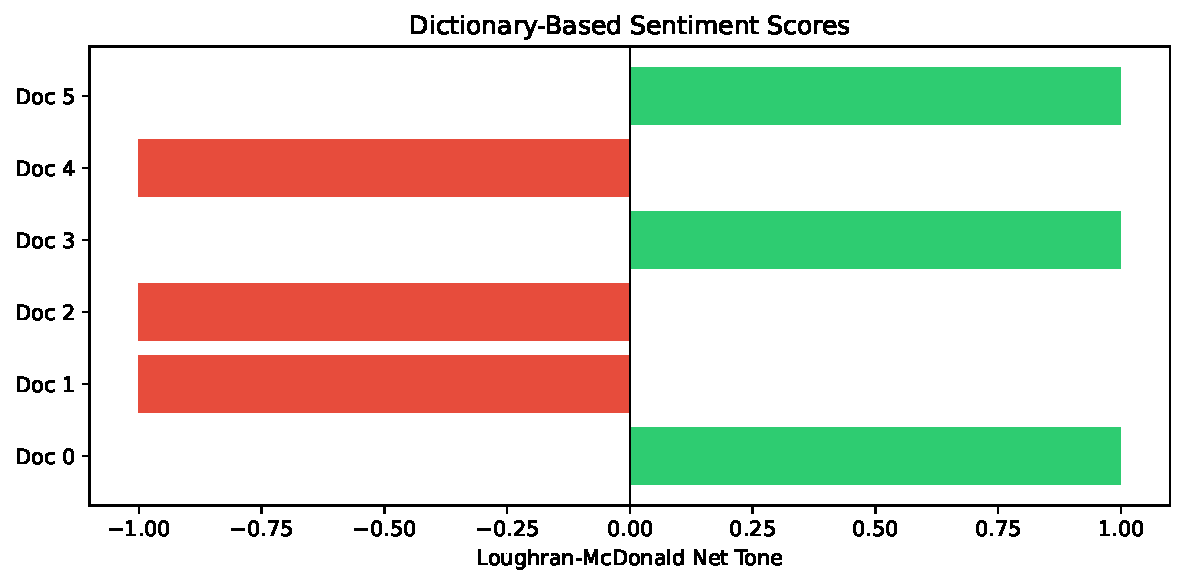
\includegraphics[width=0.7\linewidth]{files/figure_20_2_lm_score-b86dd1881505c7ad3da996bd7c706f84.pdf}

FIGURE 20.2 (panel a): dictionary-based sentiment scores for six KO-style sentences. Positive tone is shown in green, negative in red. Doc 2 illustrates the negation problem: a positive statement (``losses did not materialize, margins held firm'') receives a strongly negative score because the dictionary sees ``losses'' but cannot read ``did not materialize.''

The visualization in FIGURE 20.2 (panel a) makes the limitations of the dictionary approach immediately apparent. While the method works well for straightforward sentences, it systematically misclassifies negated statements. In Chapter 22, we will see that transformer-based models handle negation naturally through contextual representations.

\paragraph{From sentiment scores to factor signals}

The seminal application of textual sentiment to asset pricing is \cite{tetlock2007giving}, who studied the ``Abreast of the Market'' column in the Wall Street Journal. Using the Harvard GI to measure the fraction of negative words, Tetlock found that high media pessimism predicted downward pressure on market prices, followed by a reversion to fundamentals. Crucially, the effect was concentrated in small stocks with high individual investor ownership, consistent with a behavioral explanation in which noise traders overreact to negative tone.

This finding opened a productive line of research. \cite{tetlock2008more} extended the analysis to firm-level news and showed that the fraction of negative words in stories about individual firms predicted lower subsequent earnings, suggesting that journalists incorporate fundamentally relevant information. \cite{loughran2011liability} refined the measurement using their domain-specific dictionary and confirmed that negative tone in 10-K filings predicts higher post-filing return volatility, lower earnings, and wider bid-ask spreads. \cite{engelberg2011causal} pushed the literature a step further on causal identification: they used weather-driven disruptions to local newspaper delivery as an instrument and showed that local press coverage of S\&P 500 earnings announcements roughly doubles local trading activity, providing direct evidence that the media is not merely reporting prices but shaping them. \cite{hillert2014media} then connected sentiment to a classical anomaly by showing that firms with high media coverage exhibit substantially stronger momentum returns, with the effect largest for glamour stocks followed by many journalists, suggesting that press attention amplifies the behavioural frictions that sustain cross-sectional momentum.

To construct a news-tone factor for the cross-section, one typically proceeds as follows:

\begin{enumerate}
\item For each firm $n$ at time $t$, collect all relevant text documents (news articles, filings, transcripts) published during the period $(t -1, t]$.
\item Compute a sentiment score for each document using Equation (20.3) or a variant.
\item Aggregate across documents, possibly weighting by recency or source prominence, to obtain a firm-level sentiment signal $s_{t,n}$.
\item Use $s_{t,n}$ as a cross-sectional factor alongside the traditional characteristics from Chapter 1.
\end{enumerate}

To make the factor scale-invariant across periods we standardize the score cross-sectionally each rebalancing date,

\begin{equation}
z_{t,n} = \frac{s_{t,n} - \mu_t}{\sigma_t}, \quad \mu_t = \frac{1}{N_t}\sum_{n=1}^{N_t} s_{t,n}, \quad \sigma_t^2 = \frac{1}{N_t}\sum_{n=1}^{N_t} (s_{t,n} - \mu_t)^2
\tag{20.4}
\end{equation}

where the cross-section at date $t$ has $N_t$ firms. The portfolio implementation that we use throughout this chapter is the equal-weighted long-short \textit{decile spread},

\begin{equation}
r^{\text{LS}}_{t \to t+h} = \frac{1}{|\mathcal{D}_t^{10}|}\sum_{n \in \mathcal{D}_t^{10}} r_{t \to t+h, n} - \frac{1}{|\mathcal{D}_t^{1}|}\sum_{n \in \mathcal{D}_t^{1}} r_{t \to t+h, n}
\tag{20.5}
\end{equation}

with $\mathcal{D}_t^{10}$ and $\mathcal{D}_t^{1}$ the top and bottom deciles of $z_{t,n}$, and $r_{t \to t+h, n}$ the $h$-period total return on firm $n$. The cross-sectional information coefficient at horizon $h$, which we report extensively in the case study of Chapter 24, is the Spearman rank correlation between the standardized signal and the forward return computed within each cross-section and then averaged across dates,

\begin{equation}
\text{IC}(h) = \frac{1}{T}\sum_{t=1}^{T} \rho^{\text{Spearman}}\!\left(\{z_{t,n}\}_{n=1}^{N_t},\, \{r_{t \to t+h, n}\}_{n=1}^{N_t}\right).
\tag{20.6}
\end{equation}

Equations (20.4) through (20.6) supply the language we need to compare sentiment methods quantitatively: an information coefficient and a decile-spread Sharpe are the two summary statistics that the empirical tables of Chapter 21 and the case study of Chapter 24 are organized around.

The aggregation step is important and non-trivial. \cite{calomiris2019news} showed that \textit{novelty-weighted} sentiment, which down-weights language that merely repeats prior disclosures, is more informative for predicting returns than raw sentiment. The intuition is simple: a 10-K filing that repeats last year's risk factors verbatim contains less new information than one with substantially revised language.

The choice of aggregation window is equally consequential. \cite{hafez2012short} constructed several variants of a firm-level sentiment index from a commercial firm-level news sentiment dataset on a universe of 4,144 US stocks over 2000 to 2011, comparing absolute (net positive minus negative news count) and relative (positive share of total) measures across 1-day, 7-day, and 90-day rolling windows. They found that the 90-day window dominates: it smooths transient noise and captures the slower-moving component of sentiment that is most strongly associated with future returns. Using their preferred event-level score with a 90-day window, the average 3-day return spread between firms with positive and negative sentiment changes reaches 1.39\%, with most of the divergence occurring on the day the news is released. A long-short strategy built on this signal generates information ratios of 2 to 3 and a daily hit ratio close to 60\% before transaction costs. These figures should be read with the usual caveats (in-sample tuning, look-ahead in the universe construction, and gross-of-cost performance), but they illustrate a robust pattern: properly aggregated firm-level sentiment carries information beyond the contemporaneous return. An early explicit demonstration of this came from \cite{zhang2010trading}, who combined blog and news sentiment from a broad online corpus and showed that the resulting aggregate signals could be converted into profitable daily trading strategies across a large equity universe; their results were noisy at the individual-stock level but robust in aggregate, reinforcing the case for the cross-sectional sorting approach described above.

\paragraph{Limitations of dictionary methods}

Dictionary-based sentiment analysis is transparent, fast, and reproducible. It is also fundamentally limited by what we might call \textit{context blindness}. A dictionary treats each word independently, ignoring the syntactic and semantic structure of the sentence.

The most frequently cited limitation is \textbf{negation}. The sentence ``The company did not experience any significant losses'' is objectively positive, yet a dictionary approach that counts ``losses'' as negative and ignores ``not'' will assign a negative score. Various heuristic fixes exist (e.g., flipping the polarity of sentiment words that follow a negation cue within a fixed window), but they are fragile and incomplete.

\textbf{Intensifiers and diminishers} pose a related problem. ``Slightly disappointing'' and ``extremely disappointing'' carry very different magnitudes, but a dictionary assigns both the same polarity. Similarly, \textbf{conditional and hypothetical language} is common in financial text: ``If revenue were to decline, the company might need to restructure'' expresses a possibility, not a fact, yet a dictionary would count ``decline'' and ``restructure'' as negative.

\textbf{Sarcasm and implicit sentiment} are rare in formal financial documents but appear in social media and analyst commentary. A tweet reading ``Great job losing another billion dollars'' is clearly negative, but a dictionary would score ``great'' as positive.

Finally, \textbf{domain drift} is a practical concern. Language evolves, and the connotations of words change over time. A dictionary compiled from 1990s filings may not accurately capture sentiment in 2020s filings that discuss ``pandemic,'' ``supply chain disruptions,'' or ``generative AI.'' This static nature is a fundamental limitation that motivates the data-driven approaches of Chapters 21 through 23. \cite{lis2024investor} provides a useful perspective on how much of this gap has actually been closed: reviewing 71 empirical studies of investor sentiment in asset pricing models published between 2000 and 2021, the author documents that more complex sentiment measures do not reliably translate into better return prediction, and that survey-based, lexicon-based, and transformer-based signals often sit within overlapping error bars once implementation frictions are accounted for. The implication is not that modern methods are useless, but that the marginal gain per unit of modelling effort is smaller than the headlines of individual papers suggest.

A concrete out-of-sample replication of the central \cite{loughran2011liability} claim is available on a single large-cap name from the case-study corpus, KO. We score the prepared-remarks bucket of 68 KO earnings calls covering October 2006 through February 2026 with four sentiment methods (Harvard General Inquirer, the pre-LM baseline used by \cite{tetlock2007giving}; the LM dictionary; VADER, the rule-based lexicon of \cite{hutto2014vader}; and FinBERT, included here as a contextual-encoder benchmark that anticipates Chapter 22), and regress the resulting per-call score on the five-day post-call cumulative abnormal return (CAR) computed against the S\&P 500 ETF (SPY).

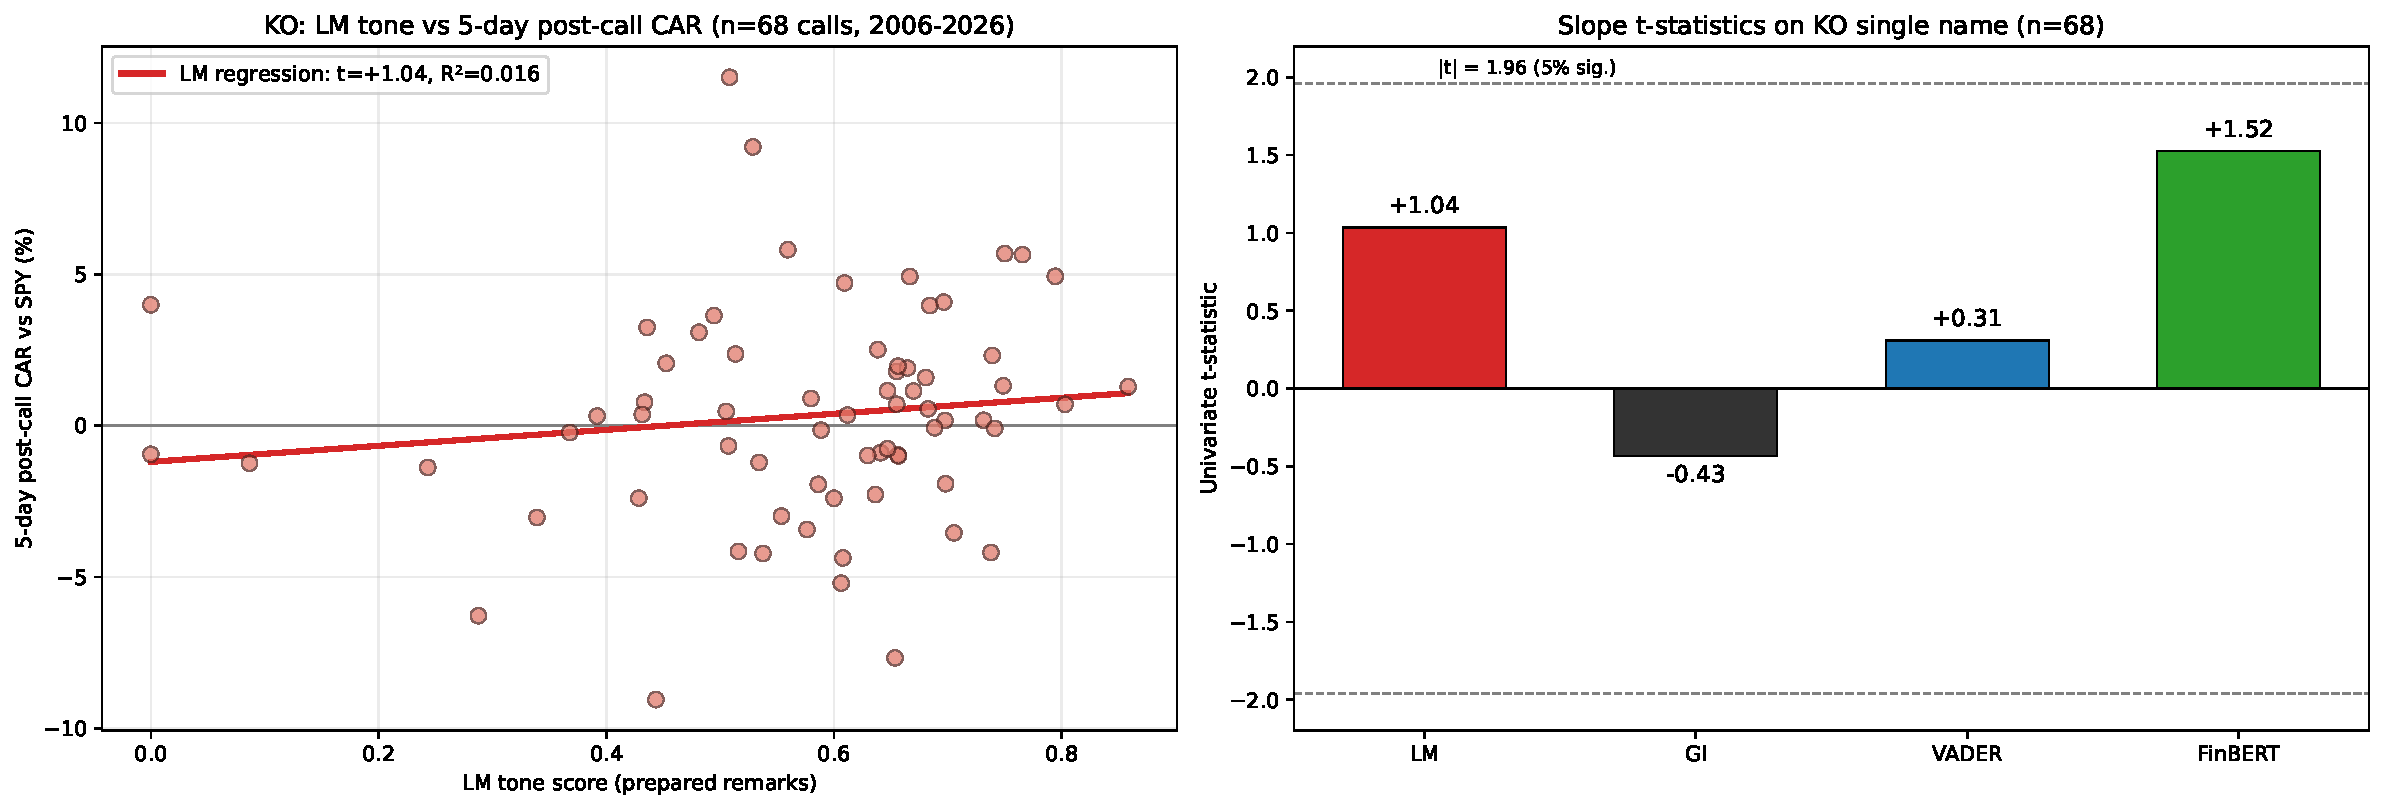
\includegraphics[width=0.7\linewidth]{files/figure_20_2b_ko_lm_r-8f34f57fa12d5e7bd12da50466e4057a.pdf}

Panel (b) of FIGURE 20.2 (KO single-name replication): the left sub-panel shows the scatter of KO five-day post-call CAR against the prepared-remarks LM tone, with the OLS regression line and its t-statistic. The right panel reports the slope t-statistics of the same regression for all four methods. On this single-name sample (n=68), LM achieves a univariate t-statistic of +1.04 with R\textsuperscript{2}=0.016, ahead of GI at -0.43 and VADER at +0.31. FinBERT, the only contextual-encoder method in the comparison, leads at t=+1.52 with R\textsuperscript{2}=0.034. None of these four single-name slopes is statistically significant at the 5\% level (|t|\textless 1.96), which is exactly the point: at a single large-cap name there is simply too little variation across 68 calls for any sentiment method to clear conventional significance, regardless of how sophisticated the model is. What the figure does illustrate is the \textit{qualitative} hierarchy that recurs at scale: LM outranks GI on the sign of the slope (consistent with the \cite{loughran2011liability} thesis that finance-domain dictionaries beat generic ones), and FinBERT in turn outranks LM (consistent with the contextual-encoder lift documented in Chapter 22).

\subsubsection{Topic modeling}

\paragraph{Latent Dirichlet Allocation}

While sentiment analysis reduces text to a single dimension (positive vs. negative), many financial applications require a richer representation that captures \textit{what} the text is about, not just its tone. \textit{Topic models} provide such a representation by discovering latent thematic structure in a corpus.

The most widely used topic model is \textbf{Latent Dirichlet Allocation} (LDA), introduced by \cite{blei2003latent}. The generative story behind LDA is elegant:

\begin{enumerate}
\item Each document is a mixture of $J$ latent topics, with mixing proportions $\boldsymbol{\theta}_d \sim \text{Dir}(\boldsymbol{\alpha})$.
\item Each topic $j$ is a distribution over the vocabulary, $\boldsymbol{\phi}_j \sim \text{Dir}(\boldsymbol{\beta})$.
\item For each word position in document $d$:

\begin{itemize}
\item Draw a topic assignment $z \sim \text{Multinomial}(\boldsymbol{\theta}_d)$.
\item Draw a word $w \sim \text{Multinomial}(\boldsymbol{\phi}_z)$.
\end{itemize}
\end{enumerate}

The Dirichlet priors $\boldsymbol{\alpha}$ and $\boldsymbol{\beta}$ control the sparsity of the topic mixtures and word distributions, respectively. A small $\alpha$ encourages documents to concentrate on a few topics; a small $\beta$ encourages topics to concentrate on a few words.

Formally, the joint distribution of a corpus of $D$ documents, given hyperparameters $\boldsymbol{\alpha}$ and $\boldsymbol{\beta}$, factorizes as

\begin{equation}
p(\mathbf{w}, \mathbf{z}, \boldsymbol{\theta}, \boldsymbol{\phi} \mid \boldsymbol{\alpha}, \boldsymbol{\beta}) = \prod_{j=1}^{J} p(\boldsymbol{\phi}_j \mid \boldsymbol{\beta}) \prod_{d=1}^{D} p(\boldsymbol{\theta}_d \mid \boldsymbol{\alpha}) \prod_{n=1}^{N_d} p(z_{d,n} \mid \boldsymbol{\theta}_d)\, p(w_{d,n} \mid \boldsymbol{\phi}_{z_{d,n}})
\tag{20.7}
\end{equation}

where $N_d$ is the length of document $d$ and $w_{d,n}, z_{d,n}$ are the $n$-th word and its latent topic assignment. Posterior inference targets the marginal $p(\mathbf{z} \mid \mathbf{w}, \boldsymbol{\alpha}, \boldsymbol{\beta})$, which has no closed form; in practice we estimate it by collapsed Gibbs sampling or variational Bayes. The key output for financial applications is the document-topic matrix $\boldsymbol{\Theta} \in \mathbb{R}^{D \times J}$, where $\theta_{d,j}$ represents the proportion of document $d$ that belongs to topic $j$. These topic proportions can serve directly as features in a factor model.

\paragraph{Financial applications}

Topic models have found several applications in equity investing. We highlight two prominent examples.

\textbf{Risk theme discovery.} \cite{israelsen2014does} applied LDA to the risk-factor sections (Item 1A) of 10-K filings and discovered interpretable risk themes such as ``litigation risk,'' ``regulatory risk,'' ``commodity price risk,'' and ``technology risk.'' Firms with high exposure to specific risk topics exhibited different return patterns, suggesting that topic proportions capture economically meaningful variation in firm-level risk that is not fully captured by traditional factors.

\textbf{Text-derived factors beyond Fama-French.} \cite{lopezlira2023risk} used topic models on news articles to construct text-based factors and showed that these factors span a significant portion of the cross-sectional variation in returns. The key insight is that topics capture latent themes (e.g., ``energy crisis,'' ``trade war,'' ``pandemic recovery'') that cut across traditional sector and style classifications.

The number of topics $J$ is a hyperparameter that must be chosen by the researcher. Common choices range from 10 to 50, depending on the granularity desired. Model selection criteria such as perplexity and topic coherence scores (\cite{roder2015exploring} survey the space of coherence measures) provide quantitative guidance, but human inspection of the top words per topic remains essential.

To make this concrete, we fit an LDA model to a small corpus of financial news headlines. In a production setting, the corpus would be much larger (thousands of articles per month), and the number of topics would be tuned using coherence metrics.

\begin{verbatim}
from sklearn.decomposition import LatentDirichletAllocation
from sklearn.feature_extraction.text import CountVectorizer

headlines = [
    "Federal Reserve raises interest rates by 25 basis points",
    "Oil prices surge amid Middle East tensions",
    "Tech stocks rally on strong earnings from Apple and Microsoft",
    "GDP growth slows as consumer spending weakens",
    "Central bank signals pause in monetary tightening cycle",
    "Crude oil futures fall on rising US production",
    "NASDAQ hits record high driven by AI chip demand",
    "Unemployment claims rise signaling labor market cooling",
    "European Central Bank holds rates steady citing inflation concerns",
    "Semiconductor stocks jump after strong guidance from NVIDIA",
    "Housing starts decline as mortgage rates reach 20-year high",
    "Gold prices rise as investors seek safe haven assets",
    "Retail sales disappoint raising recession fears",
    "Natural gas prices drop on mild winter forecasts",
    "Bond yields fall as markets price in rate cuts",
]

np.random.seed(42)
count_vec = CountVectorizer(
    stop_words='english',                            # Remove English stop words
    max_features=50                                  # Limit vocabulary size
)
dtm = count_vec.fit_transform(headlines)
\end{verbatim}

\begin{verbatim}
lda = LatentDirichletAllocation(
    n_components=3,                                  # Number of topics
    random_state=42,
    max_iter=20
)
topic_proportions = lda.fit_transform(dtm)

vocab = count_vec.get_feature_names_out()
for j in range(3):
    top_idx = lda.components_[j].argsort()[-6:][::-1]
    top_words = [vocab[i] for i in top_idx]
    print(f"Topic {j}: {', '.join(top_words)}")
\end{verbatim}

\begin{verbatim}
Topic 0: prices, rise, stocks, strong, haven, investors
Topic 1: oil, bank, central, european, holds, inflation
Topic 2: rates, fall, high, housing, decline, 20
\end{verbatim}

The topics are only partially interpretable, which is itself the lesson of running LDA on a corpus this small. Topic 2 is the cleanest: it groups the rate-and-macro headlines (the Fed hike, the GDP slowdown, housing starts, retail sales, and bond yields all load on it most heavily). Topic 1 collects energy and central-bank vocabulary (oil, crude, and the European Central Bank), and Topic 0 gathers an equities-and-safe-haven cluster (stocks, strong guidance, gold, and safe-haven demand). The separation is imperfect, with several headlines splitting their mass across topics, because fifteen short headlines give the model too little co-occurrence evidence to carve clean themes; the same procedure on tens of thousands of documents produces the sharp, stable topics that the technique is known for. We visualize the topic proportions for each headline in FIGURE 20.3.

\begin{verbatim}
fig, ax = plt.subplots(figsize=(10, 6))
im = ax.imshow(topic_proportions, aspect='auto', cmap='YlOrRd')
ax.set_yticks(range(len(headlines)))
ax.set_yticklabels([h[:50] + '...' if len(h) > 50 else h
                     for h in headlines], fontsize=8)
ax.set_xticks(range(3))
ax.set_xticklabels(['Equities/Haven', 'Energy/CB', 'Rates/Housing'])
ax.set_xlabel('Topic')
plt.colorbar(im, ax=ax, label='Topic proportion')
ax.set_title('LDA Topic Proportions for Financial Headlines')
plt.tight_layout()
plt.show()
\end{verbatim}

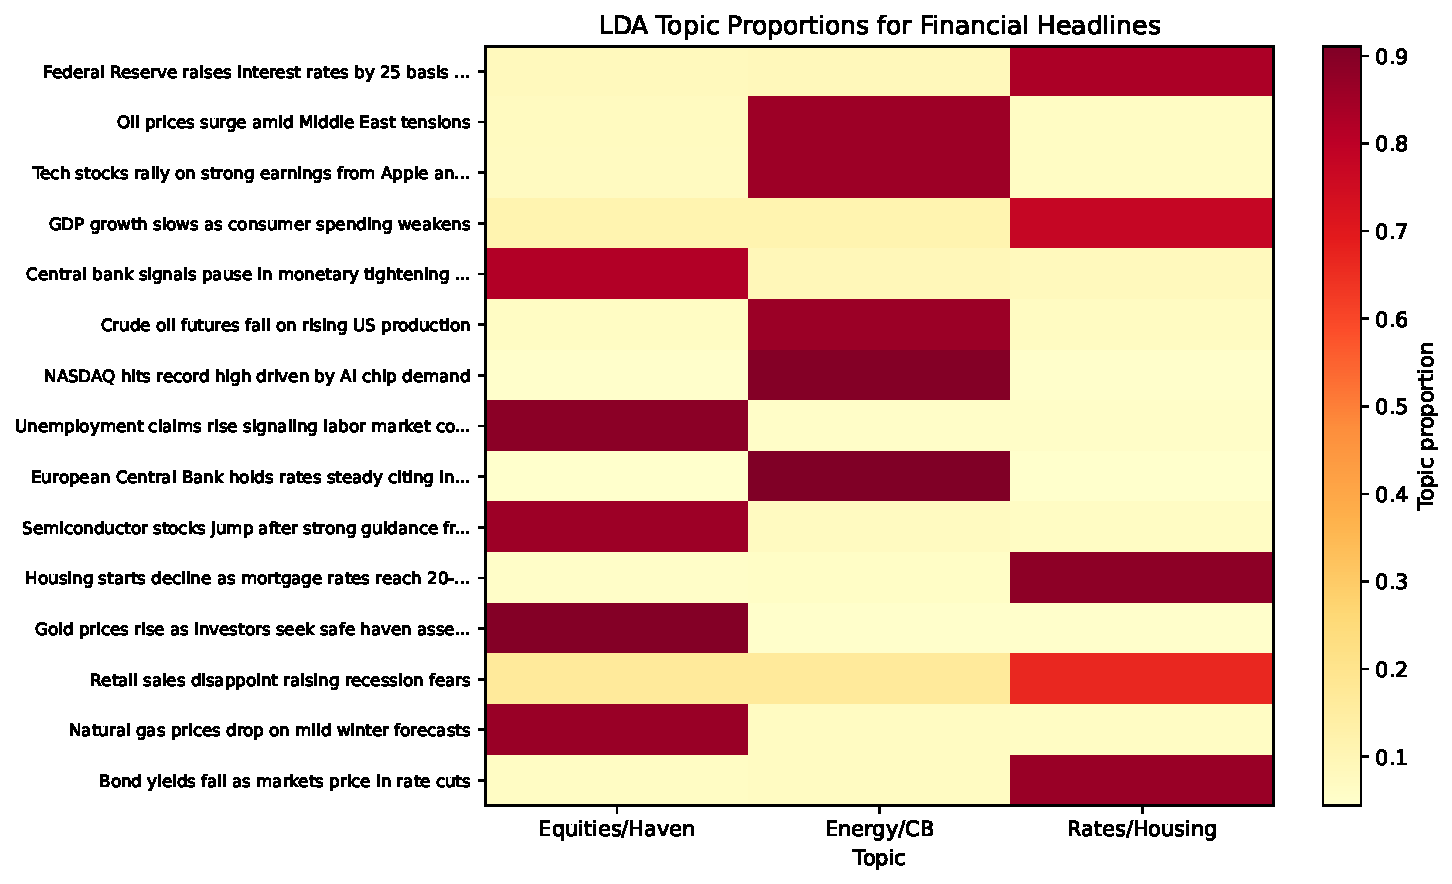
\includegraphics[width=0.7\linewidth]{files/figure_20_3_lda_heat-e9a6882d26eb6734a43933822ad956c3.pdf}

LDA topic proportions for 15 financial headlines. Each row shows the estimated mixture of three topics for one headline. The three columns correspond to the equities-and-safe-haven, energy-and-central-bank, and rates-and-housing clusters identified above.

The heatmap in FIGURE 20.3 shows how each headline distributes its mass across the three topics. The rate-and-macro headlines load most heavily on Topic 2, as expected: ``Federal Reserve raises interest rates'', ``Housing starts decline as mortgage rates reach 20-year high'', and ``Bond yields fall as markets price in rate cuts'' all peak there. The energy headlines (``Oil prices surge'', ``Crude oil futures fall'') concentrate on Topic 1, and the equities headlines (``Gold prices rise as investors seek safe haven assets'', ``Semiconductor stocks jump'') on Topic 0, though several headlines spread their proportions fairly evenly, a direct visual signal of the weak topic separation that a fifteen-document corpus produces.

\paragraph{Extensions}

Two extensions of standard LDA deserve mention. \textbf{Dynamic topic models} \citep{blei2006dynamic} allow topic distributions to evolve over time, which is natural for financial applications where the salience of themes (e.g., ``pandemic,'' ``inflation,'' ``AI'') changes across market regimes. \textbf{Structural topic models} (STM) introduced by \cite{roberts2014structural} incorporate document-level metadata (e.g., publication date, firm sector, filing type) as covariates that influence the topic proportions. This allows the researcher to ask questions such as ``Do firms in the energy sector discuss regulatory risk more than firms in technology?'' while controlling for other observable characteristics. A further extension is to couple topic assignments with sentiment scoring rather than treating the two as independent pipelines. \cite{nguyen2015topic} showed, in the context of social-media message-board posts, that conditioning sentiment on the latent topic (their Joint Sentiment-Topic model, TSLDA) substantially improves next-day return-direction prediction relative to topic-agnostic sentiment; the intuition is that the word ``risk'' carries very different valence in a macro-rates discussion than in an earnings-surprise thread. This topic-conditioned sentiment approach anticipates the contextualised representations produced by word embeddings (§20.7) and, ultimately, by transformer models (§20.11), where meaning is determined jointly by the word and its full surrounding context.

\subsubsection{Named entity recognition and event extraction}

\paragraph{Principle}

While sentiment and topics capture the tone and theme of text, many financial applications require identifying specific entities and events mentioned in documents. \textit{Named entity recognition} (NER) is the task of locating and classifying named entities in text into predefined categories such as persons, organizations, locations, dates, and monetary values.

For financial text, relevant entity types include:

\begin{itemize}
\item \textbf{Organizations:} company names, ticker symbols, regulatory bodies.
\item \textbf{Persons:} CEO names, board members, central bank officials.
\item \textbf{Monetary values:} deal sizes, revenue figures, price targets.
\item \textbf{Dates:} earnings dates, merger deadlines, policy meeting dates.
\item \textbf{Events:} mergers and acquisitions, CEO departures, product launches, regulatory actions.
\end{itemize}

NER enables structured information extraction from unstructured text. For example, given the headline ``Microsoft acquires Activision Blizzard for USD 68.7 billion,'' an NER system identifies ``Microsoft'' and ``Activision Blizzard'' as organizations, ``USD 68.7 billion'' as a monetary value, and the entire sentence as describing an acquisition event. This structured output can then be linked to firm identifiers in a financial database.

The \texttt{spaCy} library ships pre-trained NER pipelines that resolve this example out of the box. The small English model (\texttt{en\_core\_web\_sm}) is sufficient for short headlines and runs in milliseconds; the larger transformer-based pipeline (\texttt{en\_core\_web\_trf}) is more accurate on long, jargon-heavy financial prose but slower.

\begin{verbatim}
import spacy                                     # install: pip install spacy
                                                 #          python -m spacy download en_core_web_sm
nlp = spacy.load('en_core_web_sm')               # small English pipeline
headline = ("Microsoft acquires Activision Blizzard for USD 68.7 billion, "
            "with the deal expected to close by June 30, 2024.")
doc = nlp(headline)
for ent in doc.ents:
    print(f"{ent.text:25s} | {ent.label_}")
\end{verbatim}

\begin{verbatim}
Microsoft                 | ORG
Activision Blizzard       | PERSON
USD 68.7 billion          | MONEY
June 30, 2024             | DATE
\end{verbatim}

Each detected span has a \texttt{.label\_} (entity type) and character offsets into the source text. Downstream code can filter for \texttt{ORG} spans to link to ticker symbols, for \texttt{MONEY} to extract deal sizes, and for \texttt{DATE} to align the event to a calendar bar. The output also illustrates a typical failure mode: the small model misclassifies \texttt{Activision Blizzard} as \texttt{PERSON} rather than \texttt{ORG}, because the proper noun pattern matches its prior on first-last-name pairs. The larger transformer pipeline (\texttt{en\_core\_web\_trf}) usually fixes this. For finance-specific entity types not covered by the off-the-shelf models (e.g., \texttt{CUSIP}, \texttt{ISIN}, distinct CEO roles), or to harden the recall on company names like the one just misclassified, the spaCy \texttt{EntityRuler} lets one inject regex- or gazetteer-based rules ahead of the statistical NER component; the resulting hybrid pipeline keeps the recall of the pretrained model and adds the precision of hand-curated patterns for the long-tail entities that matter for equity research.

\paragraph{Applications in equity research}

NER and event extraction support several equity research workflows:

\textbf{Building event databases.} By systematically applying NER to news feeds, researchers can construct databases of corporate events (M\&A announcements, CEO changes, patent filings, lawsuits) at a scale and speed that would be impossible manually. These event databases enable event studies in the tradition of \cite{mackinlay1997event} and event-driven trading strategies.

\textbf{Entity-level sentiment.} In a news article that mentions multiple companies, the overall sentiment of the article may differ from the sentiment associated with each individual firm. For example, ``Apple's gain is Samsung's loss'' is positive for Apple but negative for Samsung. Entity-level sentiment links the tone of specific sentences to the firms they mention.

\textbf{Supply chain and network analysis.} By extracting company mentions and their relationships from news and filings, researchers can map supply chain networks, competitive relationships, and industry linkages. \cite{hoberg2016text} used textual similarity of 10-K business descriptions as a measure of product market proximity, constructing ``text-based network industries'' that outperform SIC and NAICS codes for predicting cross-sectional returns.

\textbf{Knowledge graphs as factor sources.} A more ambitious use of entity extraction is to build a \textit{knowledge graph}: a directed graph whose nodes are companies, people, products, events, and abstract concepts, and whose edges are co-mentions, supplier-customer relationships, partnerships, or thematic exposures extracted from news and filings at scale. Each security can then be assigned a set of \textit{concept exposure} scores that measure how strongly it is connected (directly or indirectly) to a given concept, and aggregated to the cross-section those scores become a candidate factor. Knowledge-graph signals are fundamentally complementary to the bag-of-words and transformer-based features discussed in Sections 20.3 to 20.6: they operate on structured relationships extracted from text rather than on the text itself, and their alpha depends on the quality of entity disambiguation and edge construction rather than on sentiment lexicons or contextual embeddings. The peer-reviewed empirical literature on stand-alone KG-derived factors is comparatively thin and is dominated by work that feeds the graph into a downstream predictor rather than using concept exposures directly. A natural extension of this entity-extraction pipeline to patent filings, cross-referencing entity mentions with the USPTO patent database, would enable the text-based novelty factors of \cite{kogan2017technological} to be constructed algorithmically at scale, though this application is outside the scope of the current chapter.

As a worked example of entity extraction, we demonstrate NER using the \texttt{spaCy} library, which provides pre-trained models for English text.

\begin{verbatim}
import spacy                                         # Industrial-strength NLP

nlp = spacy.load('en_core_web_sm')                   # Load small English model

text = ("On January 15, 2024, Microsoft Corporation announced "
        "the completion of its $68.7 billion acquisition of "
        "Activision Blizzard. CEO Satya Nadella stated that "
        "the deal would strengthen Microsoft's position in "
        "the gaming industry. Shares of Microsoft rose 2.3% "
        "following the announcement.")

doc = nlp(text)
print(f"{'Entity':<25s} {'Label':<12s} {'Description'}")
print("-" * 60)
for ent in doc.ents:
    print(f"{ent.text:<25s} {ent.label_:<12s} {spacy.explain(ent.label_)}")
\end{verbatim}

\begin{verbatim}
Entity                    Label        Description
------------------------------------------------------------
January 15, 2024          DATE         Absolute or relative dates or periods
Microsoft Corporation     ORG          Companies, agencies, institutions, etc.
$68.7 billion             MONEY        Monetary values, including unit
Activision Blizzard       ORG          Companies, agencies, institutions, etc.
Satya Nadella             PERSON       People, including fictional
Microsoft                 ORG          Companies, agencies, institutions, etc.
2.3%                      PERCENT      Percentage, including "%"
\end{verbatim}

The NER model correctly identifies all key entities: the date of the announcement, the organizations involved (Microsoft, Activision Blizzard), the CEO's name, the deal value, and the stock price change. In a production pipeline, these extracted entities would be linked to a master security database (mapping ``Microsoft Corporation'' and ``Microsoft'' to the same ticker MSFT) and stored in a structured event table for downstream analysis.

\subsubsection{Disclosure-based factors}

Corporate disclosures, 10-K and 10-Q filings, and earnings-call transcripts give rise to a self-contained family of equity factors built directly on the language of those documents. The signals reviewed below are not NLP-flavoured versions of value or quality factors; they are anomalies in their own right, identified by the accounting-finance literature and indexed by what the disclosure says, by how it is written, by what has changed in it relative to prior periods, and by what management chooses to discuss on the associated conference call. We organise the subsection around four mechanisms, readability and obfuscation, deceptive language, lazy-prices-style disclosure changes, and structured transcript analytics, and close with the quantity dimension of disclosure.

\textbf{Readability and obfuscation.} \cite{li2008annual} showed that annual report readability, measured by the Fog Index (a function of average sentence length and the proportion of complex words), predicts subsequent earnings. Less readable filings are associated with lower and more volatile future earnings, consistent with the hypothesis that managers strategically obscure bad news through complex language. The Fog Index has since been used as a quality signal in factor models: firms with unusually opaque filings may be concealing deteriorating fundamentals. \cite{bushee2018linguistic} refined the interpretation by decomposing linguistic complexity in firm disclosures into an \textit{obfuscation} component (complexity that managers use to conceal unfavourable information) and an \textit{information} component (complexity that reflects the genuine difficulty of the underlying economics). They show that only the obfuscation component is associated with lower trading volume and higher bid-ask spreads around 10-K filings, while the information component actually helps analysts incorporate complex facts into their forecasts. For factor investors, the practical lesson is that raw Fog Index scores can be noisy as stand-alone signals, and benefit from being residualised against proxies for business complexity before being used as a quality input.

\textbf{Deceptive language.} \cite{larcker2012detecting} analyzed the linguistic content of CEO and CFO presentations during earnings conference calls and identified markers of deceptive language: executives who are subsequently found to have misstated earnings use fewer self-references (``I''), more general knowledge references (``as you know''), and more extreme positive emotion words. While these signals are too noisy for stand-alone trading strategies, they can augment traditional quality metrics (such as accruals and earnings persistence) to flag firms with elevated accounting risk.

A complementary out-of-sample illustration comes from \cite{faccia2024fraud}, who applied the off-the-shelf TextBlob polarity and subjectivity scorers to the annual reports of three well-known accounting failures, Wirecard, Tesco, and Under Armour, across a multi-year window straddling each fraud period, with each firm's pre-fraud years used as its own baseline. The case-by-case trajectories are instructive precisely because they are \textit{heterogeneous}. Tesco's polarity rose from around 0.11 in the three years preceding the GBP 263 million profit overstatement to 0.148 in the 2014 fraud year, and its subjectivity rose alongside it (from roughly 0.37 in 2011-2012 to 0.60 in 2013 and 0.46 in 2014), an inflated-optimism pattern that is consistent with the deliberate-framing reading of \cite{larcker2012detecting}. Wirecard's polarity stayed essentially flat around 0.07 across 2014-2018, with only a marginal dip in the 2018 fraud year, suggesting that long-running accounting manipulation can coexist with linguistically unremarkable annual reports. Under Armour's polarity dipped in 2014 (a year before the 2015-2016 SEC investigation window) and then drifted back up across the fraud years, producing no monotonic relationship to the timing of the manipulation. The cross-section of three cases is much too small for inferential claims, but the pattern reinforces the \cite{larcker2012detecting} caveat that polarity-based forensic signals are too noisy to operate standalone: directional inferences from a single firm's tone trajectory point in opposite directions across firms. What the exercise does suggest is that forensic NLP and quality factors share a common substrate, and that a scalable version of the Faccia et al. study (thousands of restatements, automated extraction, and a within-firm pre-event baseline of the kind the paper constructs for each case) is an obvious complement to accruals-based accounting-quality scores.

\textbf{Lazy prices and disclosure changes.} \cite{cohen2020lazy} documented one of the cleanest and most surprising text-based anomalies in the accounting-finance literature. They argued that investors pay insufficient attention to year-over-year \textit{changes} in the language of 10-K and 10-Q filings, a behavioural phenomenon they call ``lazy prices''. Using a simple cosine-similarity measure between successive filings from the same firm, they sorted stocks into quintiles of textual change and found that a long-short portfolio buying firms whose filings barely changed and selling firms whose filings changed the most earned roughly 188 basis points per month, or about 22\% per year, net of standard factor exposures. The effect is concentrated in the negative tail: large text changes, which typically coincide with newly disclosed risks or litigation, are followed by persistent underperformance that takes several months to impound into prices. \cite{cohen2020lazy} further isolate the mechanism. The predictability is concentrated in changes within the Risk Factors and Management Discussion and Analysis sections of the 10-K, and especially in changes that mention executive turnover (CEO or CFO transitions), litigation, or Loughran-McDonald negative-sentiment words; the 188 basis-point monthly alpha quoted above is in fact strongest when the sort is restricted to changes in the Risk Factors section alone (t-statistic of 2.76 over their 1995-2014 sample), and changes that explicitly reference litigation and lawsuits underperform the non-changers by roughly 71 basis points per month on their own. The asymmetry is striking: roughly 86 percent of substantive year-over-year changes carry a negative-sentiment loading, while the 14 percent that read positively predict significantly \textit{positive} future returns, so the long-short result is driven by a specific tilt toward newly disclosed negative information rather than by aggregated text churn. The same construction predicts future earnings surprises, future news announcements, and even firm-level bankruptcies, anchoring the return predictability in real operational realisations rather than in a pure mispricing artefact. In practice the cosine-similarity-plus-sort construction is built on TF-IDF or document-embedding representations of the filings (see Section 20.7) rather than on raw binary word vectors, and the sorting step is combined with the usual industry and size controls.

\textbf{Systematic transcript analytics.} A more recent illustration of how structured NLP pipelines can extract multiple independent signals from the same call is provided by \cite{hafez2021transcripts}, who used a transcripts archive (roughly 500,000 conference-call documents from 2003 to 2021) to construct three orthogonal indicators: an \textit{event sentiment} score that aggregates the tone of key events detected in the call, a \textit{document sentiment} score obtained by applying a sentence-level machine learning classifier across the full transcript, and a \textit{transparency} score that counts the number of market-moving events disclosed by management. On the US universe, the document sentiment signal alone delivered information ratios above 1.1 for mid/large-cap and above 2.0 for small-cap names over holding periods of a few days to a week, and combining the three signals into a single strategy lifted these figures to 1.4 and 2.3, respectively. Two conclusions generalize beyond this particular study. First, the same transcript can support multiple largely orthogonal factors (event-level tone, document-level tone, and disclosure intensity), so researchers should resist the temptation to collapse text into a single sentiment scalar. Second, transcript signals are largely additive to news-based signals: overlaying transcripts on a standalone news-analytics strategy improved the US information ratio across nearly all holding periods, consistent with the view that earnings calls carry information that does not fully propagate into daily news flow.

\textbf{Quantity-of-disclosure factors.} Beyond tone and readability, the \textit{quantity} of disclosed text is informative in its own right. \cite{campbell2014information} study the mandatory Item 1A risk-factor disclosures introduced by the SEC in 2005 and show that firms tailor their disclosure language to their actual risk profile rather than rely on boilerplate: longer risk-factor sections are associated with higher market beta, higher idiosyncratic volatility, wider bid-ask spreads, and stronger post-filing return volatility, and the \textit{categorical} content of disclosed risks (financial, legal, tax, systematic) maps in cross-section to the corresponding realised risk dimensions. \cite{kravet2013textual} examine the complementary investor-reaction side and report that year-over-year \textit{changes} in risk-disclosure length are positively associated with post-filing increases in market-implied volatility, with the trading-volume reaction around the 10-K filing date, and with the dispersion of analyst forecasts. Newly added risk factors drive the response more strongly than restated language, an attention pattern that echoes the \cite{cohen2020lazy} ``lazy prices'' mechanism reviewed earlier in this subsection. The practical implication for factor construction is that both the level and the year-over-year change in risk-section length carry information, and that any text-quantity factor should be controlled for industry and filing-date effects to absorb the secular upward drift in 10-K length that the broader disclosure literature has documented.

\subsubsection{News and media-flow factors}

News articles, financial-media coverage, and the broader flow of public information about firms give rise to a second self-contained family of equity factors, distinct in mechanism and information horizon from the disclosure-based signals of Section 20.7. The constituent signals are constructed from the tone, volume, and breadth of media coverage rather than from corporate documents themselves, and they enter factor portfolios on their own merits, not as text-based proxies for price-based momentum. The natural reference benchmark for these signals is the price-driven momentum factor of Chapter 3, against which the news-based variant is shown to carry independent information; the rest of this section traces that argument from the early single-source evidence to the recent multi-source pipelines.

\cite{tetlock2007giving} established that media pessimism predicts negative returns, particularly for small stocks. \cite{garcia2013sentiment} extended this finding using a century of financial news data and showed that the predictive power of sentiment is concentrated in recessions, when investor uncertainty is highest. \cite{chan2003stock} found that stocks with news (regardless of tone) exhibit momentum, while stocks without news tend to show reversals.

These findings suggest that \textit{news-driven} and \textit{price-driven} return predictability (Chapter 3) capture partially distinct phenomena. A factor strategy that goes long in stocks with positive recent news sentiment and short in stocks with negative sentiment generates returns that are not fully explained by traditional momentum factors. \cite{heston2017news} confirmed this using a large dataset of news articles tagged with firm-level sentiment: news-based predictability is strongest at the weekly frequency and decays over one to two months.

The breadth of the underlying news source matters as much as the modeling choice. \cite{hafez2014web} compared a sentiment indicator built on Dow Jones newswires alone with one built on a broader corpus of more than 22,000 web publications, applied as an overlay on a short-term reversal strategy on the Russell 3000. The two sources prove complementary: Dow Jones is timelier (60 to 80\% of novel stories appear before the market open, against less than 50\% on the web) and dominates regulatory and credit-related categories, while the web edition is broader for operational news and stabilizes monthly company coverage near 95\%. Adding web content to the Dow Jones signal lowers signal turnover and lifts the information ratio of the combined strategy by up to 70\%. A second result is more sobering: the predictive content of the sentiment indicator is concentrated in small and mid-cap names. The 10-day return spread between the top and bottom sentiment quintiles reaches roughly 0.38\% on Russell 2000 stocks but is statistically indistinguishable from zero on Russell 1000 stocks, consistent with the view that large-cap prices already impound public news efficiently. Practitioners should therefore restrict text-based momentum strategies to the segment of the cross-section where news travels slowly enough to be tradable.

\textbf{News-implied volatility.} A different slice of the same media-sentiment literature focuses on text as a proxy for macro uncertainty rather than firm-level tone. \cite{manela2017news} built a monthly \textit{news-implied volatility} (NVIX) index that spans more than a century, from 1890 to 2009, by training a support-vector regression on the front-page text of the Wall Street Journal and using the fitted model to reconstruct a VIX-like uncertainty measure in the pre-option era. Two headline findings emerge from their analysis. First, NVIX has substantial out-of-sample explanatory power for the realised VIX over the short post-1986 window in which both series exist, with out-of-sample $R^2$ on the order of 0.2. Second, a one-standard-deviation increase in NVIX predicts an excess return on the aggregate US market of roughly 3.3\% over the following twelve months, consistent with a variance-risk-premium interpretation in which text-based uncertainty is compensated in expected returns. The broader point for factor investors is that text can proxy for a \textit{latent} state variable (here, uncertainty) whose own numerical proxy is only available for a fraction of the sample, extending classical time-series tests into pre-option-market history without relying on volatility data that did not exist.

\subsubsection{Coding exercises}

\begin{enumerate}
\item Download the Loughran-McDonald sentiment word lists from the authors'
website. Apply the dictionary to a set of 10-K filing excerpts (available
from SEC EDGAR) and compute the net tone for each filing. Group the
filings by sector and compare the distribution of sentiment scores
across sectors. Do some sectors systematically exhibit more negative tone?
\item Using the \texttt{gensim} library, train an LDA topic model with 10 topics on a
corpus of at least 500 financial news headlines (e.g., from a public
dataset on Kaggle). Inspect the top-10 words for each topic and assign
interpretable labels. Then merge the topic proportions as features in a
simple return prediction model (e.g., linear regression) and evaluate
whether any topics have significant predictive power for next-month
returns.
\end{enumerate}

\subsubsection{References}